		\begin{enumerate}
			\item
			\begin{enumerate}
				\item $(A(0),B(0)) = (0,1)$
				\item The solution is periodic because $(A(0),B(0))=(A(8),B(8))$
				\item \phantom{x}

				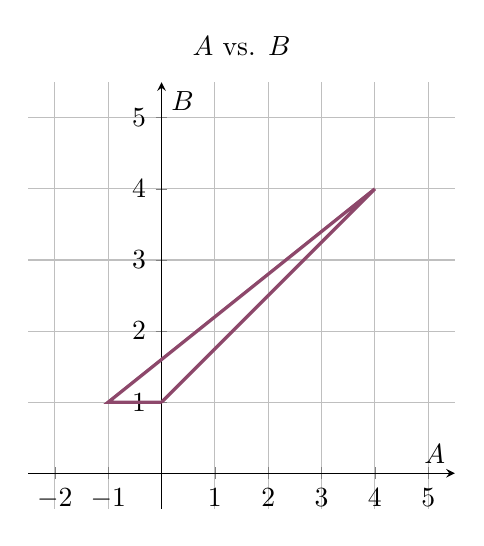
\begin{tikzpicture}
					\begin{axis}[
						title={$A$ vs. $B$},
						width=7cm,
						height=7cm,
						xmin=-2.5,xmax=5.5,
						ymin=-.5,
						ymax=5.5, xmajorgrids, ymajorgrids,
						xtick={-10,...,10}, ytick={0,1,...,10},
						axis lines=middle,
						samples=5, domain=-5:5,
						xlabel={$A$},
						ylabel={$B$}
						]
						
						%\addplot[red, thick] coordinates {(0,0) (2,4) (5,-1) (8,0)};
						%\addplot[green!50!black, thick] coordinates {(0,1) (2,4) (5,1) (8,1)};
						\addplot[magenta!50!black, very thick] coordinates {(0,1) (4,4) (-1,1) (0,1)};
					\end{axis}
				\end{tikzpicture}%
				
			\end{enumerate}
			\item \begin{enumerate}
				\item \phantom{x}

				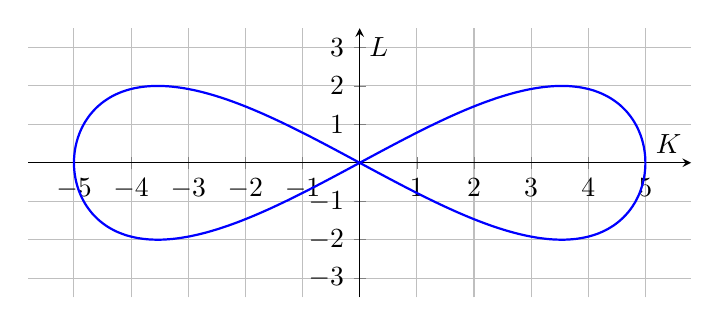
\begin{tikzpicture}
					\begin{axis}[
						width=10cm,
						height=5cm,
						xmin=-5.8,xmax=5.8,			
						ymin=-3.5,
						ymax=3.5, xmajorgrids, ymajorgrids,
						xtick={-5,...,5}, ytick={-10,...,10},
						axis lines=middle,
						samples=5, domain=-5:5,
						xlabel={$K$},
						ylabel={$L$}
						]
						
						\addplot [
							domain=0:2*pi,
							samples=100,
							smooth,
							thick,
							blue
						] 
						({5*sin(deg(x))}, {2*sin(deg(2*x))});
					\end{axis}
				\end{tikzpicture}%
			\end{enumerate}

			\item By definition, if $\vec u\in\Span(Y)$, then $\vec u=\alpha_1\vec y_1+\cdots+\alpha_4\vec y_4$.
				By distributivity of the dot product, we have
				\[
					\vec x\cdot \vec u = \vec x\cdot (\alpha_1\vec y_1+\cdots+\alpha_4\vec y_4)
					=\alpha_1(\vec x\cdot \vec y_1)+\cdots +\alpha_4(\vec x\cdot \vec y_4)=0,
				\]
				so $\vec x$ is orthogonal to every vector in $\Span(Y)$.

			\item \begin{enumerate}
				\item $\ell_1$ and $\ell_2$ are close and $\ell_3$ and $\ell_4$ are close.
				\item $\vec n_1\approx\mat{-0.70711\\0.70711}$,
					$\vec n_2\approx\mat{-0.70675\\0.70746}$,
					$\vec n_3\approx\mat{-0.0005\\1}$, and $\vec n_4\approx\mat{-0.0003\\1}$.
				\item
					$\|\vec n_1-\vec n_2\|\approx 0.0005$,
					$\|\vec n_1-\vec n_3\|\approx \|\vec n_1-\vec n_4\|
					\approx \|\vec n_2-\vec n_3\|\approx \|\vec n_2-\vec n_4\|\approx 0.765$,
					and
					$\|\vec n_3-\vec n_4\|\approx 0.0017$.

					These distances coincide with my intuitive idea of closeness. Using normal
					vectors might be preferable to using direction vectors, because it generalizes to
					planes. A plane has a unique
					normal direction but infinitely many direction vectors that might be hard to compare.
			\end{enumerate}
		\end{enumerate}